% Short paper skeleton. Build: cd paper/short && latexmk -pdf main.tex
% Full draft (2026-11-19), written by Claude from the author's dictation and the results; the author edits.
% Numbers are from results/RESULTS.md; check any change against it.
% Body target: 4 pages (abstract to the end of Section 5). References and appendix do not count.
% For a venue, swap the documentclass/style for its template; the content does not depend on it.
\documentclass[11pt]{article}
\usepackage[margin=1in]{geometry}
\usepackage[T1]{fontenc}
\usepackage[utf8]{inputenc}
\usepackage{lmodern,microtype,amsmath,amssymb,graphicx,booktabs,xcolor}
\usepackage[numbers,sort&compress]{natbib}
\usepackage[hidelinks]{hyperref}

\definecolor{slotred}{HTML}{B3261E}
\definecolor{slotgrey}{HTML}{55554F}
% \slot{word budget}{facts to carry}: a red box for the author's text.
\newcommand{\slot}[2]{\par\smallskip\noindent\fcolorbox{slotred}{white}{\begin{minipage}{0.97\linewidth}
  \small\textcolor{slotred}{\textbf{Your text, about #1 words.}}\par\color{slotgrey}\footnotesize #2\end{minipage}}\par\smallskip}

\title{The Unread Map: LLMs Encode Spatial Geometry but Answer From the Text}
\author{Cristhian G\'omez Neira}
\date{}

\begin{document}
\maketitle

\begin{abstract}
Humans solve geometry problems with the help of mental images. We ask whether large language models build an internal
geometric representation from text, and whether they use it to answer. A short text places three objects on a plane,
each relative to the previous one, and asks which of the first and the last is farther east or north; the answer
needs both steps. Gemma 3 12B answers from the last sentence alone: when the first step is larger and points the
other way, it is right on 0.34 of questions, below chance. Yet the model combines the two steps and carries the
result to where the answer is written: a linear probe there answers the same questions correctly (0.86 against the
model's 0.32; in Gemma 3 27B, 0.98 against 0.25). About twenty late components write the shortcut while others damp
it, and in 12B removing them reveals no correct answer underneath. The map is built but not read, and the gap grows
with size. All tests were preregistered.
\end{abstract}

\section{Introduction}
% Draft from the author's dictation (2026-11-19). Edit freely.
Humans represent geometric objects in their minds, and in a sense they can see them. When we solve a problem that
involves geometry, we do not only use the axioms and the text of the problem: we represent each object and, in a way,
see it. A transformation, a movement, a position on a map: each is represented visually. People rotate imagined
objects at a steady rate \citep{shepard1971rotation} and scan an imagined map in a time that grows with the distance
\citep{kosslyn1978scanning}.

The question of this paper, and of the series it starts, is whether LLMs do something similar: whether they represent
geometry internally in a way that helps them solve these problems. The question has two parts. A representation is
\emph{present} if the information can be decoded from the model's activations. It is \emph{used} if changing that
information changes the answer. The debate on mental imagery in psychology was about the second part, not the first
\citep{kosslyn1978scanning,pylyshyn2002imagery}. In LLMs, probes have found space, time and the state of a board game
\citep{gurnee2023space,li2023othello}, but information that can be decoded is not always used
\citep{ravichander2021probing,orgad2025know}.

We test both parts on the simplest case we could build. A text places three objects on a plane, each relative to the
previous one: R, then M relative to R, then C relative to M. We ask which is farther east (or north), C or R. The
answer needs both steps. It also has a shortcut: the direction of C's own sentence, which gives the right answer
unless M's step is larger and points the other way. On those questions, a model that reads its map is right and a
model that takes the shortcut is wrong.

We study Gemma 3 12B and 27B \citep{gemma2025gemma3}, and preregister every test. We find:
\begin{itemize}\setlength\itemsep{0pt}
  \item \textbf{The model takes the shortcut.} When M's step is larger and points the other way, Gemma 3 12B is right
    on 0.34 of questions, below chance.
  \item \textbf{The geometry is there.} The model combines the two sentences into C's position and carries the
    information to the position where the answer is written. There, a linear probe answers those same questions
    correctly: 0.86 against the model's 0.32 (12B), 0.98 against 0.25 (27B).
  \item \textbf{A few late components write the answer.} Attention heads in the last layers read C's direction from the
    question and vote for it, while other components damp the vote. Removing the 20 strongest voters, and nothing
    else, does not reveal a correct answer underneath: accuracy rises only to 0.46. Giving them the values of a flipped
    question flips 98\% of the answers when only C moves.
  \item \textbf{The gap grows with size.} In 27B the probe is better and the model worse; the shortcut is written by
    more components, so removing 20 of them is not enough there.
\end{itemize}

The map is built and carried to the answer, but not read: the failure is in the read-out, not in building the map.
This paper tests the simplest case, three objects on a plane; the next papers in the series go further.

\section{Setup}
\paragraph{Task.} Each prompt describes three objects, one sentence each. Every object is placed relative to the
previous one by whole units east or west and north or south. The list of objects and a question follow:
\begin{quote}\small
Beth is 4 units east of Amy. Leo is 1 unit west of Beth. The objects are: Leo, Beth, Amy.
Which is farther east, Leo or Amy? Answer with one word.
\end{quote}
We call the objects R (Amy), M (Beth) and C (Leo). On the asked axis, $d_1$ is M's step from R and $d_2$ is C's own
step from M; C is the correct answer if $d_1+d_2>0$. In the example $d_1=4$ and $d_2=-1$: Leo is farther east, but
Leo's own sentence says west. We group the questions by how the two steps combine: \emph{own step only} ($d_1=0$),
\emph{agree}, \emph{first step only} ($d_2=0$), and two kinds of conflict, \emph{C larger} and \emph{M larger}. The
last is the decisive case: there the rule ``C if its own sentence points the asked way'' gives the wrong answer. Names
are single tokens (people or objects); questions ask about east or north and name C or R first, balanced.

\paragraph{Models and measure.} Gemma 3 12B and 27B instruct (48 and 62 layers), in bfloat16. The model's answer is
the sign of $\mathrm{logit}(C)-\mathrm{logit}(R)$ at the final position.

\paragraph{Methods.} \emph{Probes} are ridge regressions on the residual stream, fitted and tested on different
scenes. \emph{Copying} replaces the activation at one site and layer with its value in a run where one step points
the other way; the share of the full effect each copy carries shows where the information flows. The \emph{logit
lens} reads the C-vs-R logit difference at each layer. \emph{Direct attribution} splits the final logit difference
exactly into the contributions of each attention head, MLP and the embeddings, through Gemma's normalisations (the
parts sum to the model's logit difference, $r=1.000$). \emph{Twin-mean removal}: every question has a twin, the same
question with C's step negated; a component's output at the final position is replaced by the average of its outputs
on the question and its twin. This removes what follows C's direction and keeps the names and everything else. The
\emph{shortcut} is the coefficient of own\_yes (C's step points the asked way) in a regression of the logit difference
on own\_yes, the correct answer, $d_1$, $d_2$ and the name order; the correct answer is in the regression so that a
read-out turning towards it is not counted as shortcut. Every test and decision rule was preregistered
(Appendix~\ref{app:prereg}).

\section{Results}

\begin{figure}[t]
  \centering
  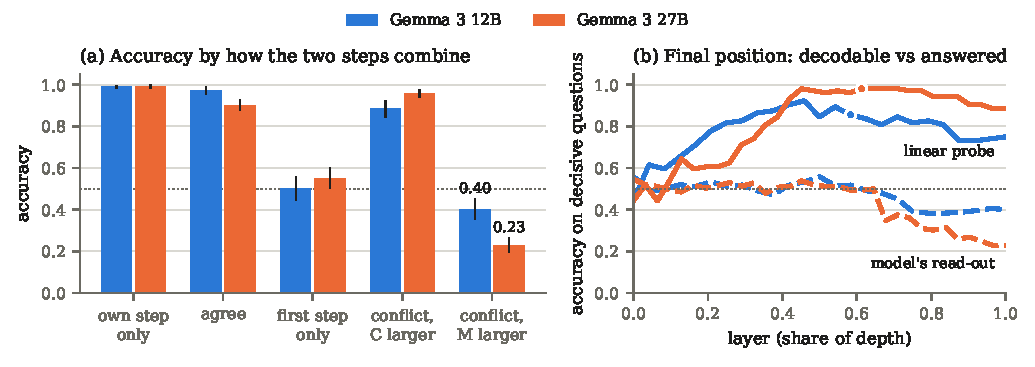
\includegraphics[width=\linewidth]{figures/fig1_behaviour_probe.pdf}
  \caption{Behaviour, and what the answer position holds. (a) Accuracy by how the two steps combine on the asked
  axis, for the same 2,400 questions in both models; error bars are 95\% scene-bootstrap intervals, the dotted line
  is chance. (b) Decisive questions only (M's step larger and opposite). Solid: a linear probe for the correct answer
  at the final position, tested on held-out scenes. Dashed: the model's own answer read at that layer (logit lens).
  Layers are shown as a share of depth.}
  \label{fig:behaviour}
\end{figure}

\subsection{The model answers from one sentence}
Figure~\ref{fig:behaviour}a shows accuracy by case. Both models are right on 0.89 to 0.99 of the questions where C's
own sentence gives the answer (own step only, agree, conflict with C's step larger) and at chance where only M's
sentence does (first step only). When the steps conflict and M's is larger, both fall below chance: 0.40 (12B) and
0.23 (27B). A separate preregistered test on 5,250 new questions gives 0.34 [0.30, 0.37] for 12B; across all conflict
questions the model follows C's own step in 77\% of answers. The model behaves as if it answered from one sentence:
C is farther east if C's sentence says east. M's step shifts the model's confidence but rarely its answer. This is a
shortcut in the usual sense \citep{geirhos2020shortcut}: a rule that agrees with the truth on most questions and fails
exactly where both steps are needed.

\subsection{The answer position holds the right answer}
\paragraph{The model composes.} Before the question, at the end of C's own sentence (12B, layer 24), C's distance to
R can be read with $R^2=0.61$, against 0.15 for the best probe on a side-by-side code of the two sentences (gap
+0.45 [+0.38, +0.53]); on pairs of steps never seen in training, 0.51 against $-0.03$. The model does not just store
the two sentences; it combines them.

\paragraph{The information reaches the answer.} Copying activations traces both steps from their sentences to the
question tokens (12B layers 20--24, 27B layers 24--32) and then to the final position, where M's step reads with
$R^2=0.84$ (12B) and 0.89 (27B).

\paragraph{The right answer is there.} A linear probe for the correct answer at the final position, fitted on other
scenes, is right on 0.86 of the held-out decisive questions (12B, layer 28), where the model is right on 0.32; for
27B, 0.98 (layer 38) against 0.25. On first-step-only questions, where the model is at chance, the probe is right on
all of them. Figure~\ref{fig:behaviour}b shows both curves by depth. The probe rises over the first half of the
network and stays high; the model's own read-out is at chance until about 60\% of depth and then turns to the
shortcut, by layer 36 in 12B and 44 in 27B. The preregistered verdict for both models: the information reaches the
answer position, and the read-out ignores it.

\begin{figure}[t]
  \centering
  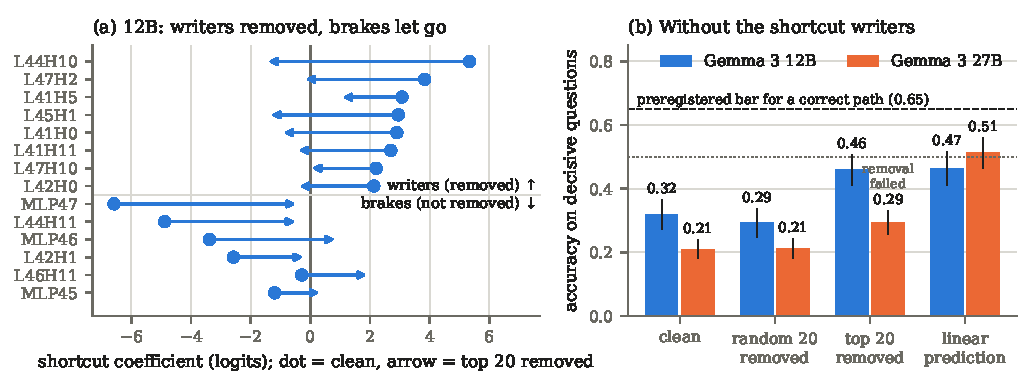
\includegraphics[width=\linewidth]{figures/fig2_mechanism.pdf}
  \caption{The components that write the answer. (a) Gemma 3 12B: each component's shortcut coefficient in the
  normal run (dot) and with the 20 strongest writers removed by twin mean (arrow head), for the 8 largest writers and
  the 6 brakes that change most. The writers lose their vote; the brakes relax towards zero. (b) Accuracy on the
  decisive questions (1,474-question test set): normal run, 20 matched random components removed, the 20 writers
  removed, and the prediction from subtracting the shortcut term. Dashed: the preregistered bar for a correct
  read-out. Error bars are 95\% scene-bootstrap intervals.}
  \label{fig:mechanism}
\end{figure}

\subsection{A few late components write the answer}
\paragraph{Writers and brakes.} We split the logit difference at the final position into the contribution of each
component and regress each contribution on the question variables. The shortcut is written by attention heads in
the last layers (12B: layers 41--47; L44H10, L47H2, L45H1, L41H0, \dots). The ten largest write +36 logits of
shortcut, the model's total is +22, and the rest of the model contributes $-14$: other components push against the
vote. We call them brakes. The writers read the question tokens, where C's direction has arrived, not C's sentence.

\paragraph{Removing the writers.} Replacing these heads by their average output does not remove the shortcut. They
copy names, so their average adds a bias that depends on which names C and R are (81--86\% of the change it causes),
and the shortcut comes back in full (preregistered verdict: ineffective). We therefore remove only what follows C's
direction, with the twin mean. With the top 20 components removed, the shortcut falls from 20.3 to 6.2 [4.5, 8.0]
logits (20 matched random components: 28.0). If a correct read-out were hidden under the shortcut, accuracy on the
decisive questions should now rise. It rises from 0.32 to 0.46 [0.41, 0.51]: what subtracting the shortcut term alone
predicts (0.47), and far below the preregistered bar of 0.65 (Figure~\ref{fig:mechanism}b). The preregistered
verdict: no correct path underneath the shortcut.

\paragraph{These components set the answer.} Giving the 20 components their values from the twin flips the answer to
the twin's shortcut on 98\% of own-step-only questions (93--99\% in every case except agree, 72\%).

\paragraph{Self-repair is brakes letting go.} About two thirds of the removed shortcut comes back ($-46.3$ removed,
$+31.2$ back). Most of it, 78\%, comes from brakes relaxing towards zero once the vote is gone (MLP47 $-6.6\to-0.3$,
L44H11 $-4.9\to-0.3$; Figure~\ref{fig:mechanism}a), not from backup writers taking over. This resembles the backup
and negative heads of the IOI circuit \citep{wang2022ioi} and self-repair in other models
\citep{mcgrath2023hydra,rushing2024selfrepair}.

\subsection{Replication on Gemma 3 27B}
Table~\ref{tab:replication} lists the criteria, fixed before any 27B data. Layer windows were scaled to depth, and the
components were chosen by the 12B rule on 27B's own data. The behaviour and the flow of information replicate, more
strongly than in 12B (Figure~\ref{fig:behaviour}). The component-level result does not: removing the top 20 leaves
+21.9 of +36.9 logits of shortcut (0.55 of the control; the rule needs less than 0.50), and swapping them flips only
0.37 of own-step-only answers. The reason is spread, not a different mechanism. In 27B the top 20 do 56\% of all
shortcut writing, against 75\% in 12B, and 80\% of it needs 55 components, against 34. The writers sit in the same
place (layers 47--60, 76--97\% of depth), and the shortcut comes back the same way (78\% from brakes relaxing, mostly
the last MLPs). Where the shortcut is cancelled (swap, coefficient +1.0), accuracy is about 0.6, and subtracting the
shortcut term predicts 0.51 on the decisive questions: no sign of a correct path, but this part is exploratory.

\begin{table}[t]
  \centering
  \small
  \caption{Preregistered replication criteria (\texttt{docs/preregistration\_replication\_27b.md}, committed before
  any 27B data).}
  \label{tab:replication}
  \begin{tabular}{@{}lccc@{}}
    \toprule
    criterion & 12B & 27B & holds \\
    \midrule
    shortcut: accuracy on conflict, M larger $<0.5$ & 0.40 & 0.23 & yes \\
    flow map: reaches the answer position, read-out ignores it & yes & yes & yes \\
    removing the top 20 shows no correct path underneath & yes & ineffective (0.55 $>$ 0.50) & no \\
    swapping the top 20 sets the answer ($\ge 0.80$, own step only) & 0.98 & 0.37 & no \\
    \bottomrule
  \end{tabular}
\end{table}

\section{Related work}
\paragraph{Represented is not used.} Probing accuracy does not show that a model uses the information
\citep{ravichander2021probing}, and LLMs can encode the correct answer and still generate a wrong one
\citep{orgad2025know}. In models trained from scratch on one task the decoded world state is used: editing
Othello-GPT's board changes its moves \citep{li2023othello}. Generative models can also predict well with an
incoherent world model \citep{vafa2024world}.

\paragraph{Space in pretrained LLMs.} LLMs encode geographic coordinates and dates linearly \citep{gurnee2023space}.
Gemma 3 builds the structure of a grid presented in context but struggles to use it \citep{lepori2026incontext}.
Closest to us, \citet{ma2026lexical} find in multimodal LLMs that the correct spatial relation stays available inside
the model while a lexical bias overrides it. We show the same pattern in text, for a position the model must compose
rather than a stated relation; we locate the components that override it, show that nothing correct remains when
they are removed, and find that the gap grows with size.

\paragraph{Shortcuts and self-repair.} The shortcut fits the wider picture of shortcut learning
\citep{geirhos2020shortcut} and of LLMs that solve tasks with a bag of heuristics \citep{nikankin2025heuristics}. The
brakes and their release resemble backup and negative heads \citep{wang2022ioi} and self-repair
\citep{mcgrath2023hydra,rushing2024selfrepair}.

\section{Limitations and conclusion}
\paragraph{Limitations.} We study one model family at two sizes, in their instruct versions, and one task: three
objects on a plane and one kind of question. We intervene only at the final position; the step where C's direction
moves onto the question tokens is not tested. A linear probe shows that the information is present and bounds what a
linear read-out could achieve; it does not show that the model could learn to use it. Components were selected by
regression, and in 27B twenty are not enough to remove the shortcut.

\paragraph{Conclusion.} Gemma 3 builds the geometry: it combines two relative positions into one and carries the
result to the place where the answer is written. Then it answers from one sentence. The failure is in the read-out,
not in building the map, and a larger model builds a better map without reading it. In the terms of the imagery
debate, the image is there, but on this task it does no work. The next papers in the series test richer geometry and
ask what, if anything, makes a model read its map.

\bibliographystyle{plainnat}
\bibliography{refs}

\appendix
\section{Preregistration}\label{app:prereg}
Each design and decision rule was committed before its data
(\url{https://github.com/ccgomezn/geometry-llm}, file \texttt{docs/preregistration\_*.md}).

\begin{center}
\small
\begin{tabular}{@{}llll@{}}
  \toprule
  test & document & committed & verdict \\
  \midrule
  shortcut (5,250 questions, 12B) & \texttt{axis\_bulk} & 7a91a8d, 2026-11-14 & follows C's own step \\
  composition (12B) & \texttt{compose} & 7b5a958, 2026-11-15 & composed by the model \\
  flow map (12B) & \texttt{flow} & e550537, 2026-11-15 & reaches the answer position \\
  writers, mean ablation (12B) & \texttt{components} & bcb15f5, 2026-11-15 & ineffective \\
  writers, twin-mean removal (12B) & \texttt{components2} & 9ebc6f8, 2026-11-15 & no correct path underneath \\
  replication (27B) & \texttt{replication\_27b} & f0fbfbd, 2026-11-19 & partial (Table~\ref{tab:replication}) \\
  \bottomrule
\end{tabular}
\end{center}

\paragraph{Mean ablation.} Replacing a writer's output by its mean over questions changed the answers mostly through
the names: 81--86\% of the change it caused was explained by which names C and R were, and the shortcut coefficient
was restored in full.

\paragraph{The random control in the twin-mean test.} The matched random components include brakes (their
coefficients sum to $-3$ to $-12$ per draw), so removing them raises the shortcut to 28.0. Compared with the normal
run instead, the conclusion is the same: shortcut 20.3 to 6.2, decisive accuracy 0.32 to 0.46, with the upper bound
of its interval below 0.60.

\section*{AI assistance}
% Adapted from v1's disclosure; it applies again because Claude drafts text from the author's dictation. Edit freely.
The author used Claude (Anthropic) to help write the experiment code, run analyses, and draft and edit this text from
the author's dictated ideas. The research questions, the preregistered designs and decision rules, and the conclusions
were set and checked by the author, who takes responsibility for all content. Every number comes from the result files
in the public repository.

\section*{Code and data}
Code, preregistrations with their commit history, and all result files:
\url{https://github.com/ccgomezn/geometry-llm}. Figures: \texttt{paper/short/make\_figs.py}.

\end{document}
